%----------------------------------------------------------------------------------------
%	PACKAGES AND THEMES
%----------------------------------------------------------------------------------------
\documentclass[aspectratio=169,xcolor=dvipsnames]{beamer}
\usetheme{Antibes}
\usecolortheme{beaver} 

\usepackage[utf8]{inputenc}
\usepackage{amsmath, amsfonts, amsthm, amscd, amssymb}
\usepackage{tikz} 
\usepackage[vlined]{algorithm2e}
\usepackage{pgf,tikz}
\usepackage[english]{babel}
\usepackage{lmodern}
\usepackage[T1]{fontenc}
\usepackage{hyperref}
\usepackage{color}
\usepackage{graphicx} % Allows including images
\graphicspath{{Figures/}} %Setting the graphicspath
\usepackage{booktabs} % Allows the use of \toprule, \midrule and \bottomrule in tables
\usepackage{cancel}
\usepackage{animate}
\usepackage{array}
\usepackage{xcolor,colortbl}
\usepackage{subfigure}

% Pour les diagrams fait avec matcha
\usepackage{physics}
\usepackage{amsmath}
\usepackage{mathdots}
\usepackage{yhmath}
\usepackage{siunitx}
\usepackage{multirow}
\usepackage{gensymb}
\usepackage{tabularx}
\usepackage{extarrows}
\usetikzlibrary{fadings}
\usetikzlibrary{patterns}
\usetikzlibrary{shadows.blur}
\usetikzlibrary{shapes}


\usepackage[%backend=biber,
style = ieee,
sorting=none
]{biblatex} %,bibstyle=ieeehttps://www.overleaf.com/project/624dc5f129c1767e8bb8de67
\addbibresource{biblio.bib}
\renewbibmacro*{date}{%
  \iffieldundef{year}
    {\bibstring{nodate}}
    {\printdate}
}

% \usepackage{ulem}

\newcolumntype{a}{ >{\columncolor{blue}} c }

\setbeamertemplate{navigation symbols}{} % Remove the navigation symbols
\addtobeamertemplate{navigation symbols}{}{%
    \usebeamerfont{footline}%
    \usebeamercolor[fg]{footline}%
    \hspace{1em}%
    \insertframenumber/\inserttotalframenumber
}

\newcommand{\backupbegin}{
   \newcounter{framenumberappendix}
   \setcounter{framenumberappendix}{\value{framenumber}}
}
\newcommand{\backupend}{
   \addtocounter{framenumberappendix}{-\value{framenumber}}
   \addtocounter{framenumber}{\value{framenumberappendix}} 
}

\newcommand{\blue}[1]{\textcolor{blue!75}{#1}}
\newcommand{\green}[1]{\textcolor{teal!90}{#1}}
\newcommand{\red}[1]{\textcolor{red}{#1}}
\newcommand{\onlyred}[2]{\only<#1>{\red{#2}}}
\newcommand{\onlyblack}[2]{\only<#1>{#2}}
\newcommand{\rose}[1]{\textcolor{red!50}{#1}}


%----------------------------------------------------------------------------------------
%	TITLE PAGE
%----------------------------------------------------------------------------------------

% The title
\title[Analyse dimensionnelle : Contact de Hertz]{Analyse dimensionnelle : Contact de Hertz}
% \subtitle{Subtitle}

\author[Nous] {BRAUN-DELVOYE  Baptiste, CAN Erdi, CARTERON Augustin}
\date{6 décembre 2022} % Date, can be changed to a custom date

\institute{Sorbonne Université}

%----------------------------------------------------------------------------------------
%	PRESENTATION SLIDES
%----------------------------------------------------------------------------------------
\newcommand{\mycite}[1]{[\textcolor{blue!50}{#1}]}

\begin{document}
{
\setbeamertemplate{headline}{}
\begin{frame}
    \titlepage
    \centering
    \includegraphics[scale=.2]{SORBONNE_FAC_SCIENCES_DEF_CMJN.png}
\end{frame}
}

\begin{frame}
    \frametitle{Outline}
    \tableofcontents
\end{frame}

\section{Introduction}

\begin{frame}{Expérience}
    \begin{columns}
        \column{.6\textwidth}
        \begin{figure}
            \centering
            \includegraphics[width=0.95\textwidth]{contactHertzPhoto.png}
            \caption{Scema de notre expérience\cite{Wang2013}}
            \label{fig:wiki}
        \end{figure}
        \column{.4\textwidth}
        \begin{figure}
            \centering
            \includegraphics[height=0.7\textheight]{Figures/IMG-20221205-WA0025.jpg}
            \caption{Image de notre expérience}
            \label{fig:my_label}
        \end{figure}
    \end{columns}
\end{frame}

\begin{frame}{Les paramètres}
    \begin{itemize}
        \item Le diamètre (paramètre observable).
        \item Le poids.
        \item La masse.
        \item Module de Young.
        \item Rayon du sphère.
    \end{itemize}
    \begin{block}{Relation entre 5 paramètres dimensionnés}
        \begin{center}
            \(d_{allongé}=f(g,m,Y,r)\)
        \end{center}
    \end{block}
\end{frame}

\subsection{Théorème de Vaschy-Buckingham}
\begin{frame}{Théorème de Vaschy-Buckingham}
    \begin{columns}
        \column{.5\textwidth}
        \begin{itemize}
            \item 5 paramètres dimensionnés: d, g, m, Y, r.
            \item 3 dimensions: L, T, M.
            \item 2 nombres $\Pi$.
        \end{itemize}
        \column{.5\textwidth}
        \begin{block}{Nos nombre Pi's}   
            \begin{itemize}
                \item \(\Pi_1 = \frac{d_{allongé}}{r}\)
                \item \(\Pi_2 = \frac{Y}{g\cdot m\cdot r^{-2}}\)
            \end{itemize}
        \end{block}
    \end{columns}
\end{frame}

\section{Mesures}
\subsection{Mesures de module de Young}
\begin{frame}{Mesures de module de Young des spheres}
    \begin{columns}
        \column{.5\textwidth} 
            

\tikzset{every picture/.style={line width=0.75pt}} %set default line width to 0.75pt        

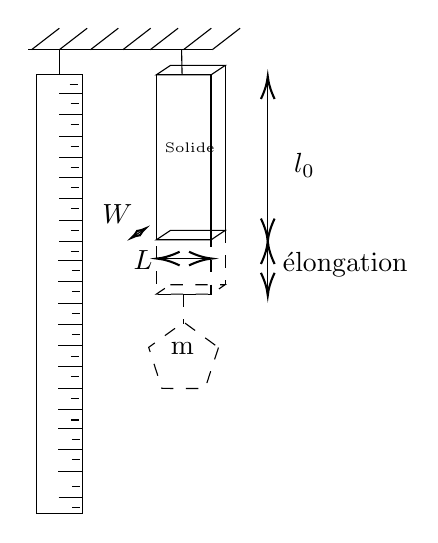
\begin{tikzpicture}[x=0.75pt,y=0.75pt,yscale=-1,xscale=1]
%uncomment if require: \path (0,280); %set diagram left start at 0, and has height of 280

%Shape: Rectangle [id:dp18040928656090194] 
\draw   (109.88,45.5) -- (136.28,45.5) -- (136.28,125) -- (109.88,125) -- cycle ;
%Shape: Rectangle [id:dp2634355860158073] 
\draw   (52,45.5) -- (74.4,45.5) -- (74.4,257) -- (52,257) -- cycle ;
%Shape: Regular Polygon [id:dp22065917641684663] 
\draw  [dash pattern={on 4.5pt off 4.5pt}] (139.86,176.87) -- (133.39,196.62) -- (112.6,196.56) -- (106.23,176.78) -- (123.08,164.61) -- cycle ;
%Straight Lines [id:da5984676937670013] 
\draw  [dash pattern={on 4.5pt off 4.5pt}]  (123.08,151.15) -- (123.08,165.61) ;
%Straight Lines [id:da7001813736123224] 
\draw    (63.2,54.5) -- (74.4,54.5) ;
%Straight Lines [id:da3062557449682686] 
\draw    (63.2,85.25) -- (74.4,85.25) ;
%Straight Lines [id:da20215985858716423] 
\draw    (63.2,75) -- (74.4,75) ;
%Straight Lines [id:da8808714878515267] 
\draw    (63.2,64.5) -- (74.4,64.5) ;
%Straight Lines [id:da6383318235924331] 
\draw    (63.2,95) -- (74.4,95) ;
%Straight Lines [id:da32883716690401354] 
\draw    (63.2,125.75) -- (74.4,125.75) ;
%Straight Lines [id:da373229105397628] 
\draw    (63.2,115.5) -- (74.4,115.5) ;
%Straight Lines [id:da1584687396901996] 
\draw    (63.2,105) -- (74.4,105) ;
%Straight Lines [id:da7512671608886448] 
\draw    (62.7,135) -- (73.9,135) ;
%Straight Lines [id:da37016590964258045] 
\draw    (62.7,165.75) -- (73.9,165.75) ;
%Straight Lines [id:da4386413017541493] 
\draw    (62.7,155.5) -- (73.9,155.5) ;
%Straight Lines [id:da02810420548527559] 
\draw    (62.7,145) -- (73.9,145) ;
%Straight Lines [id:da7697041865621039] 
\draw    (62.7,176) -- (73.9,176) ;
%Straight Lines [id:da6088947476135094] 
\draw    (62.7,206.75) -- (73.9,206.75) ;
%Straight Lines [id:da009866399889504995] 
\draw    (62.7,196.5) -- (73.9,196.5) ;
%Straight Lines [id:da21936698318722825] 
\draw    (62.7,186) -- (73.9,186) ;
%Straight Lines [id:da10738875056856667] 
\draw    (62.7,216) -- (73.9,216) ;
%Straight Lines [id:da10354569266987457] 
\draw    (62.9,248.95) -- (74.1,248.95) ;
%Straight Lines [id:da9160318279121149] 
\draw    (62.7,236.5) -- (73.9,236.5) ;
%Straight Lines [id:da8299174478560745] 
\draw    (62.7,226) -- (73.9,226) ;
%Straight Lines [id:da5682892424794057] 
\draw    (69.2,221) -- (73.1,221) ;
%Straight Lines [id:da31505228097644244] 
\draw    (69.4,253.95) -- (73.3,253.95) ;
%Straight Lines [id:da5164298144681894] 
\draw    (69.4,243.7) -- (73.3,243.7) ;
%Straight Lines [id:da11714086375901434] 
\draw    (69.2,231) -- (73.1,231) ;
%Straight Lines [id:da11091608073363757] 
\draw    (68.7,181) -- (72.6,181) ;
%Straight Lines [id:da36958078994364674] 
\draw    (68.7,211.75) -- (72.6,211.75) ;
%Straight Lines [id:da4619026429850712] 
\draw    (68.7,201.5) -- (72.6,201.5) ;
%Straight Lines [id:da21872819930489573] 
\draw    (68.7,191) -- (72.6,191) ;
%Straight Lines [id:da43941249779280755] 
\draw    (69.2,139.84) -- (73.1,139.84) ;
%Straight Lines [id:da8525442619642314] 
\draw    (69.2,170.59) -- (73.1,170.59) ;
%Straight Lines [id:da7815908650718675] 
\draw    (69.2,160.34) -- (73.1,160.34) ;
%Straight Lines [id:da816254229575871] 
\draw    (69.2,149.84) -- (73.1,149.84) ;
%Straight Lines [id:da2888918300532426] 
\draw    (68.7,99.84) -- (72.6,99.84) ;
%Straight Lines [id:da6271953850763747] 
\draw    (68.7,130.59) -- (72.6,130.59) ;
%Straight Lines [id:da41556733991066075] 
\draw    (68.7,120.34) -- (72.6,120.34) ;
%Straight Lines [id:da3258724927463501] 
\draw    (68.7,109.84) -- (72.6,109.84) ;
%Straight Lines [id:da6183762137134601] 
\draw    (68.63,59.44) -- (72.53,59.44) ;
%Straight Lines [id:da8802461831186332] 
\draw    (68.63,90.19) -- (72.53,90.19) ;
%Straight Lines [id:da9432935185644149] 
\draw    (68.63,79.94) -- (72.53,79.94) ;
%Straight Lines [id:da036904227626971986] 
\draw    (68.63,69.44) -- (72.53,69.44) ;
%Straight Lines [id:da9353346933990352] 
\draw    (68.13,50.19) -- (72.03,50.19) ;
%Shape: Rectangle [id:dp15219613954598277] 
\draw  [dash pattern={on 4.5pt off 4.5pt}] (109.88,125) -- (136.28,125) -- (136.28,151.15) -- (109.88,151.15) -- cycle ;
%Straight Lines [id:da02250764345649947] 
\draw    (163.61,127.67) -- (163.61,149.82) ;
\draw [shift={(163.61,151.82)}, rotate = 270] [color={rgb, 255:red, 0; green, 0; blue, 0 }  ][line width=0.75]    (10.93,-3.29) .. controls (6.95,-1.4) and (3.31,-0.3) .. (0,0) .. controls (3.31,0.3) and (6.95,1.4) .. (10.93,3.29)   ;
\draw [shift={(163.61,125.67)}, rotate = 90] [color={rgb, 255:red, 0; green, 0; blue, 0 }  ][line width=0.75]    (10.93,-3.29) .. controls (6.95,-1.4) and (3.31,-0.3) .. (0,0) .. controls (3.31,0.3) and (6.95,1.4) .. (10.93,3.29)   ;
%Straight Lines [id:da37635961334370194] 
\draw    (163.61,48.17) -- (163.61,123.67) ;
\draw [shift={(163.61,125.67)}, rotate = 270] [color={rgb, 255:red, 0; green, 0; blue, 0 }  ][line width=0.75]    (10.93,-3.29) .. controls (6.95,-1.4) and (3.31,-0.3) .. (0,0) .. controls (3.31,0.3) and (6.95,1.4) .. (10.93,3.29)   ;
\draw [shift={(163.61,46.17)}, rotate = 90] [color={rgb, 255:red, 0; green, 0; blue, 0 }  ][line width=0.75]    (10.93,-3.29) .. controls (6.95,-1.4) and (3.31,-0.3) .. (0,0) .. controls (3.31,0.3) and (6.95,1.4) .. (10.93,3.29)   ;
%Straight Lines [id:da7426529952875176] 
\draw    (122.08,33.37) -- (122.33,45.5) ;
%Straight Lines [id:da8220382985726795] 
\draw    (63.2,33.37) -- (63.2,45.5) ;
%Straight Lines [id:da6990307414016574] 
\draw    (48.2,33.37) -- (136.88,33.37) ;
%Straight Lines [id:da3133229244111366] 
\draw    (49.8,33.37) -- (63.2,23.02) ;
%Straight Lines [id:da6989295351103999] 
\draw    (123,33.37) -- (136.4,23.02) ;
%Straight Lines [id:da9330680403874334] 
\draw    (107,33.37) -- (120.4,23.02) ;
%Straight Lines [id:da895271983463563] 
\draw    (93.8,33.37) -- (107.2,23.02) ;
%Straight Lines [id:da30950632916719356] 
\draw    (78.2,33.37) -- (91.6,23.02) ;
%Straight Lines [id:da8439672524203561] 
\draw    (63.2,33.37) -- (76.6,23.02) ;
%Straight Lines [id:da5592106693035812] 
\draw    (136.88,33.37) -- (150.28,23.02) ;
%Shape: Rectangle [id:dp7883216139112701] 
\draw  [dash pattern={on 4.5pt off 4.5pt}] (116.69,146.59) -- (143.09,146.59) -- (136.28,151.15) -- (109.88,151.15) -- cycle ;
%Shape: Rectangle [id:dp6661452200468969] 
\draw   (116.69,120.44) -- (143.09,120.44) -- (136.28,125) -- (109.88,125) -- cycle ;
%Straight Lines [id:da5586053419576171] 
\draw    (143.09,40.94) -- (143.09,120.44) ;
%Shape: Rectangle [id:dp6444678498622427] 
\draw   (116.69,40.94) -- (143.09,40.94) -- (136.28,45.5) -- (109.88,45.5) -- cycle ;
%Straight Lines [id:da3624119912301027] 
\draw    (112.21,134) -- (134.61,134) ;
\draw [shift={(136.61,134)}, rotate = 180] [color={rgb, 255:red, 0; green, 0; blue, 0 }  ][line width=0.75]    (10.93,-3.29) .. controls (6.95,-1.4) and (3.31,-0.3) .. (0,0) .. controls (3.31,0.3) and (6.95,1.4) .. (10.93,3.29)   ;
\draw [shift={(110.21,134)}, rotate = 0] [color={rgb, 255:red, 0; green, 0; blue, 0 }  ][line width=0.75]    (10.93,-3.29) .. controls (6.95,-1.4) and (3.31,-0.3) .. (0,0) .. controls (3.31,0.3) and (6.95,1.4) .. (10.93,3.29)   ;
%Straight Lines [id:da1113209054939639] 
\draw    (103.1,120.55) -- (99.61,122.89) ;
\draw [shift={(97.95,124)}, rotate = 326.2] [color={rgb, 255:red, 0; green, 0; blue, 0 }  ][line width=0.75]    (4.37,-1.32) .. controls (2.78,-0.56) and (1.32,-0.12) .. (0,0) .. controls (1.32,0.12) and (2.78,0.56) .. (4.37,1.32)   ;
\draw [shift={(104.76,119.44)}, rotate = 146.2] [color={rgb, 255:red, 0; green, 0; blue, 0 }  ][line width=0.75]    (4.37,-1.32) .. controls (2.78,-0.56) and (1.32,-0.12) .. (0,0) .. controls (1.32,0.12) and (2.78,0.56) .. (4.37,1.32)   ;
%Straight Lines [id:da537695972291895] 
\draw  [dash pattern={on 4.5pt off 4.5pt}]  (143.09,120.44) -- (143.09,146.59) ;

% Text Node
\draw (115.67,173.33) node [anchor=north west][inner sep=0.75pt]   [align=left] {m};
% Text Node
\draw (112.74,77.06) node [anchor=north west][inner sep=0.75pt]   [align=left] {{\tiny Solide}};
% Text Node
\draw (175,82.23) node [anchor=north west][inner sep=0.75pt]    {$l_{0}$};
% Text Node
\draw (55,119.9) node [anchor=north west][inner sep=0.75pt]    {$$};
% Text Node
\draw (169.67,129.83) node [anchor=north west][inner sep=0.75pt]   [align=left] {élongation};
% Text Node
\draw (97.69,128.84) node [anchor=north west][inner sep=0.75pt]    {$L$};
% Text Node
\draw (82.67,106.94) node [anchor=north west][inner sep=0.75pt]    {$W$};


\end{tikzpicture}

        \column{.5\textwidth}
            \begin{itemize}
                \item \(\sigma = \frac{F}{S} = \frac{mg}{WL} = Y\varepsilon\)
                \item \(\varepsilon = \frac{\mathrm{élongation}}{l_0}\)
                \item \(\Longrightarrow Y = \frac{mg}{WL\varepsilon} = \frac{F}{S\varepsilon}\)
            \end{itemize}
        \end{columns}
\end{frame}

\begin{frame}
    \begin{figure}      % TODO TODO TODO nos boulles  
        \includegraphics[width = .3\textwidth]{Screenshot 2022-12-06 011933.png}
    \end{figure}
    \begin{table}[h]
        \centering
        \begin{tabular}{cccccc}
        \toprule
        %\multicolumn{1}{c}{} & \multicolumn{3}{c}{\textbf{Topic 2}} & \multicolumn{2}{c}{\textbf{Topic 3}} \\
        %\cmidrule(rl){2-4} \cmidrule(rl){5-6}
        %       v  Est il nos parametres ????
        \textbf{Parametres} & {F $\pm 0.15$ (N)} & {S \(\pm 1.5(\mathrm{mm}^2)\)} & {$\varepsilon \pm 0.01$} & {Y (Pa)} & {Y (GPa)} \\
        \midrule                                
        \rowcolor{red!10}
        Rose & 9.81 & 185.28 & 0.37 & 143099.705 & 0.00014 \\
        \rowcolor{blue!10}
        Bleu & 9.81 & 127.5  & 0.22 & 349732.620 & 0.00035 \\
        \rowcolor{green!10}
        Vert & 9.81 & 209 & 0.04 & 1173444.976 &   0.00117 \\
        \bottomrule
        \end{tabular}
    \end{table}
\end{frame}

\subsection{Mesures des diametres alonge}
\begin{frame}{Mesures des diametres alonge}
    \begin{columns}
        \column{.3\textwidth} 
        \begin{figure}
            \centering
            \includegraphics[height=0.65\textheight]{Figures/IMG-20221205-WA0025.jpg}
            \caption{Image de notre expérience}
            \label{fig:my_label}
        \end{figure}    
        \column{.3\textwidth}
        \begin{figure}
            \centering
            \includegraphics[height=0.65\textheight]{IMG-20221205-WA0027.jpg}
            \caption{Image de notre expérience}
            \label{fig:my_label}
        \end{figure}
        \column{.3\textwidth}
        \begin{figure}
            \centering
            \includegraphics[height=0.65\textheight]{IMG-20221205-WA0028.jpg}
            \caption{Image de notre expérience}
            \label{fig:my_label}
        \end{figure}
        \end{columns}
\end{frame}

% TODO metre les noms des diapos 
\section{Resultats}
\begin{frame}
    \begin{figure}
        \centering
        \includegraphics[height=0.9\textheight]{../Tous.png}
        \caption{A metre une caption} % TODO 
        \label{fig:my_label}
    \end{figure}
\end{frame}

\begin{frame}
    \begin{figure}
        \centering
        \includegraphics[height=0.9\textheight]{../Ultime.png}
        \caption{A metre une caption} % TODO 
        \label{fig:my_label}
    \end{figure}
\end{frame}

\section{La formule}
\begin{frame}{La fonction}
    \begin{block}{Fonction}
        \begin{center}
            \(d_{alongé}=1.38\cdot r\cdot\sqrt[3]{\frac{g\cdot m}{Y\cdot r^2}}=1.38\cdot \sqrt[3]{\frac{g\cdot m \cdot r}{Y}}\)
        \end{center}
    \end{block}
\end{frame}

\section{Conclusion}
\begin{frame}
    
\end{frame}


\begin{frame}[allowframebreaks,noframenumbering]{Bibliographie}
    %\thispagestyle{empty}
    \nocite{*}
    %\addcontentsline{toc}{section}{Bibliographie}
    \printbibliography[title = Bibliographie]
\end{frame}

\end{document}


